\documentclass[11pt]{article}
%\documentclass[article]{IEEEtran}
\usepackage{graphicx}
\usepackage{float}
\usepackage{amsmath}
\usepackage{amsfonts}
\usepackage[brazilian]{babel}
\usepackage[utf8]{inputenc}
\usepackage[backend=biber]{biblatex}
\usepackage{csquotes}
\usepackage{gensymb}
%\usepackage{docmute}
\usepackage{array}
\usepackage{multicol}
\usepackage{geometry}
\usepackage[T1]{fontenc}
\addbibresource{rel_final_erik_perillo_1sem2017.bib}

\newcommand{\fromeng}[1]{\footnote{do inglês: \textit{#1}}}
\newcommand{\tit}[1]{\textit{#1}}
\newcommand{\tbf}[1]{\textbf{#1}}
\newcommand{\ttt}[1]{\texttt{#1}}
\newcommand{\ie}{i.~e.~}
\newcommand{\eg}{e.~g.~}

\begin{document}

\newgeometry{margin=1.0in}

\begin{titlepage}
	\centering
	{\scshape\Large Relatório Final\par}
	\vspace{1.5cm}
	{\huge\bfseries Processos atencionais e aprendizado de máquina
		para sistemas robóticos\par}
	\vspace{1cm}
    {\itshape Aluno: Erik de Godoy Perillo (RA 135582)\par}
	{\itshape Orientadora: Profa. Dra. Esther Luna Colombini\par}
	\vspace{0.5cm}
	\vfill
    Instituto de Computação\\
	Universidade Estadual de Campinas
	\vfill
	{\large \today\par}
\end{titlepage}

\newpage

%\begin{multicols}{2}
\section{Introdução}
A capacidade de percepção e construção de um modelo da realidade ao seu redor
é fundamental para que sistemas robóticos interajam com o ambiente e executem
tarefas diversas e complexas que podem ter as mais variadas utilidades para
os humanos.
Dentro da percepção, a visão é um dos sentidos mais importantes para diversos
seres vivos (em especial aos humanos).

Um problema do sensoriamento é que nossos cérebros,
a cada segundo, recebem uma quantidade imensa de informação.
Processar todos os estímulos é uma tarefa inviável.
Um componente fundamental para lidar com esse problema é a atenção: a
habilidade de dar
foco apenas ao relevante, evitando assim o processamento desnecessário de
enormes quantias de dados.
É razoável inspirar-se na atenção para a construção de
mecanismos semelhantes que sirvam a sistemas de inteligência
artificial em máquinas.

Um conceito importante na atenção visual é a distinção
\tit{Bottom-up vs. Top-down}: Por componente \tit{bottom-up} de
atenção entende-se saliências instintivas percebidas por mudanças
e/ou contrastes muito grandes em uma cena. O componente \tit{top-down}
é aquele que dá saliência variável às \tit{features} de acordo
com a meta do agente do momento.
Neste trabalho, foca-se na atenção \tit{bottom-up}, também chamada de
saliência visual.

%Os avanços recentes em \tit{Deep Learning} levaram a modelos computacionais
%ainda mais eficientes.
A atenção tem sido foco de estudo há anos, resultando em diversas teorias
em psicologia sobre a atenção humana que inspiraram a implementação de
modelos computacionais bem sucedidos.
Duas das mais famosas teorias da psicologia sobre atenção visual
são a \tit{Feature Integration Theory} (FIT)~\cite{TreismanGelade1980} e a
\tit{Guided Search}~\cite{Wolfe1989}.
Ambas provêm contribuições importantes para o entendimento dos processos
de saliência visual
e diversos modelos computacionais foram criados baseando-se em ideias delas.
A FIT indica basicamente que se a busca de um objeto de interesse em uma
cena for por apenas uma \tit{feature}, a localização é feita em tempo
instantâneo.
Entretanto, se o objeto de interesse for composto por múltiplas \tit{features}
a serem buscadas (\eg uma linha horizontal verde),
a localização do objeto é feita em tempo linear.
Já \tit{Guided Search} diz que buscas por conjunções de \tit{features} são na
verdade mais rápidas pois a combinação das features gera um sinal de
saliência mais forte no campo visual humano.

\subsection{Mapas de saliência}
Um conceito importante no contexto de saliência visual são os mapas
de saliência (Figura~\ref{fig:salmap}).
Para cada imagem, o seu respectivo mapa de saliência é um mapa onde
regiões mais chamativas para humanos na imagem original são mais claras,
e regiões menos chamativas são mais escuras.
Tais mapas são computados a partir de observações de seres humanos feitas
nas imagens.

\begin{figure}[H]
\begin{center}
		\begin{tabular} {cc}
		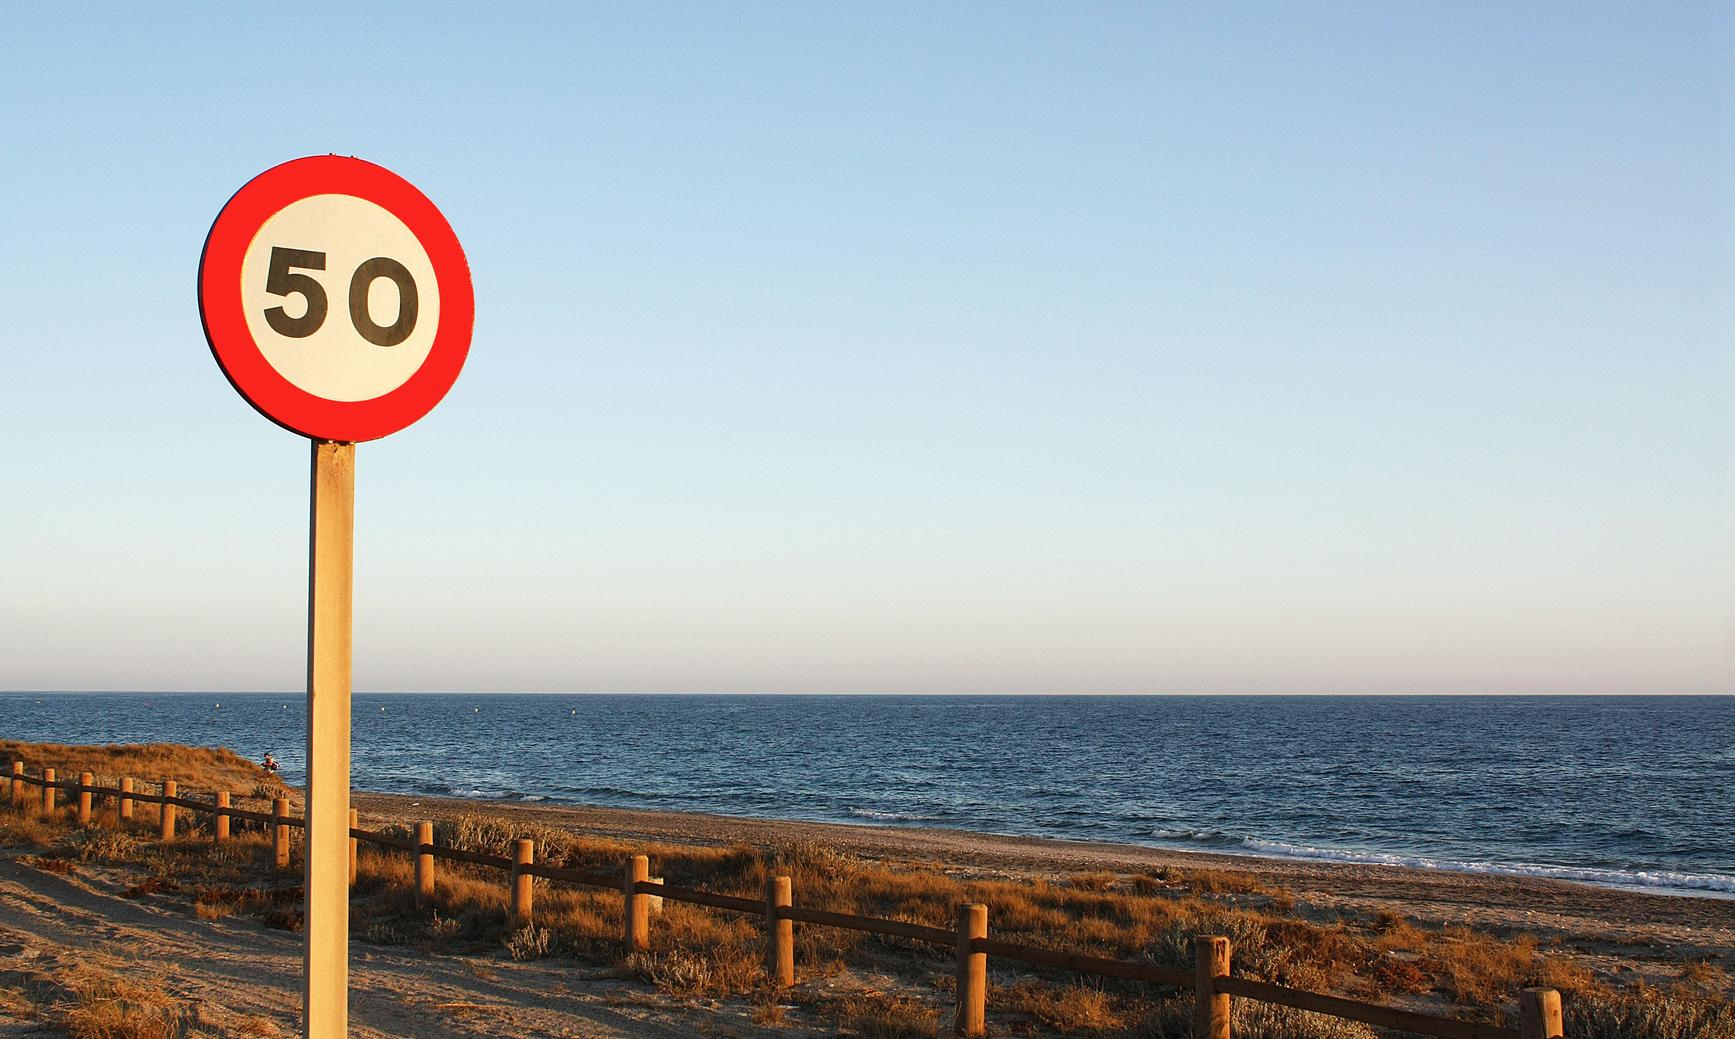
\includegraphics[width=0.45\textwidth]{./img/traffic_sign_s.jpg} &
		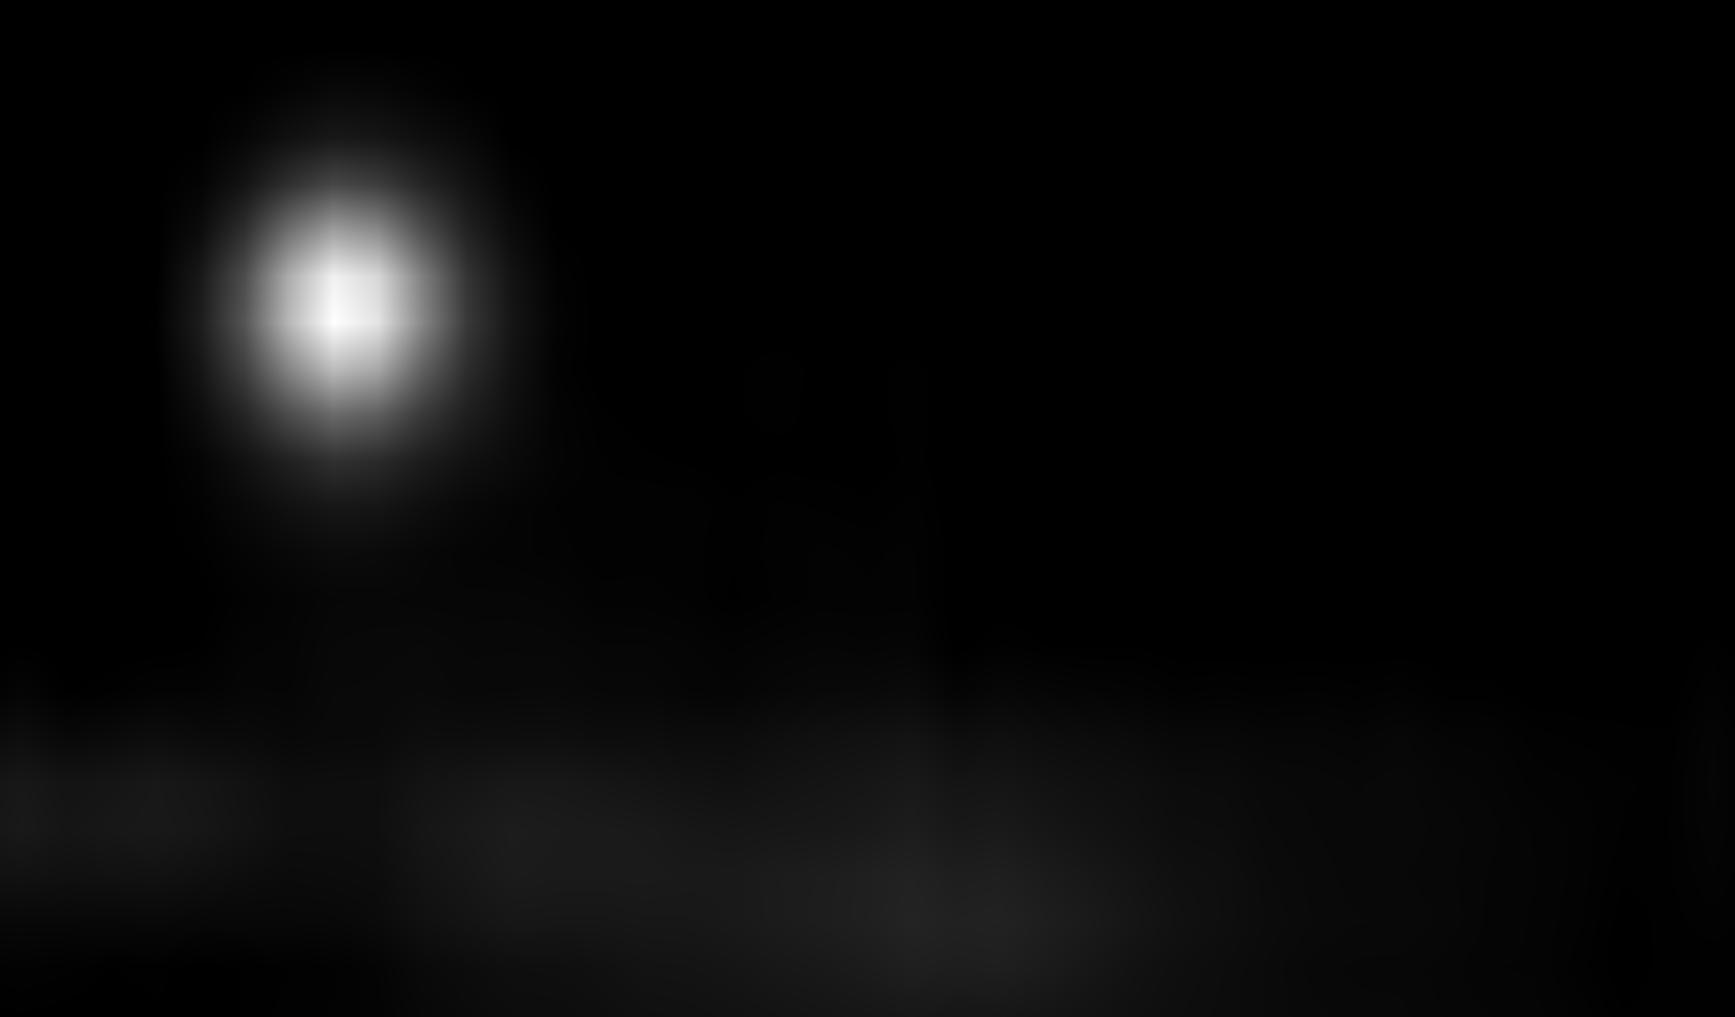
\includegraphics[width=0.45\textwidth]{./img/traffic_sign_m.jpg}\\
        (a) & (b)
		\end{tabular}
\end{center}
\caption{Exemplo de mapa de saliência. b) é o mapa de saliência onde 
    regiões mais brancas representam áreas
    mais salientes para humanos na imagem original a).}
\label{fig:salmap}
\end{figure}

\subsection{Objetivos}
Neste trabalho, objetivamos construir um modelo atencional de saliência visual que possa ser executado em um robô móvel de forma eficiente. Assim, o modelo deve ser capaz de, dada uma imagem de entrada qualquer,
produzir um mapa de saliência como o da Figura~\ref{fig:salmap}, que seja
o mais fiel possível a um mapa que seria gerado por seres humanos.
O objetivo é que o modelo possa ser usado em um \tit{framework} atencional
para robôs móveis em conjunto com outros mecanismos de atenção sensorial.

Em resumo, as principais atividades do trabalho envolvem:
\begin{itemize}
    \item Revisão bibliográfica sobre teorias sobre a atenção, principais modelos e métricas.
    \item Implementação de um modelo atencional com métodos tradicionais.
    \item Implementação de um modelo atencional com \tit{Deep Learning}, com
        eficiência suficiente para posterior uso em robôs móveis.
\end{itemize}

Cada atividade desenvolvida será mais detalhada no decorrer do documento.

\section{Materiais e métodos}
%\subsection{Modelos}

\subsection{Avaliação de desempenho}
Inicialmente, uma pesquisa sobre as métricas e \tit{datasets} mais usados para
avaliação dos modelos atencionais computacionais foi conduzida uma vez que estes pontos são imprescindíveis  para o avanço do trabalho. As métricas expressam o quão similares são os mapas de saliência gerados
por modelos computacionais em relação ao dos seres humanos (\tit{ground-truth}) enquanto os \emph{datasets} provêm a base de testes do sistema.

\subsubsection{\tit{Datasets}}
Os \tit{datasets} são compostos de imagens acompanhadas do seu conjunto-verdade,
que indica como os mapas de saliência para cada imagem deveriam ser caso fossem observados por humanos.

Dois dos principais tipos de mapas-verdade:
\begin{enumerate}
	\item Pontos de fixação de olhar: Um dispositivo de
	\tit{eye-tracking} é usado em pessoas para determinar as regiões na imagem
	onde as mesmas olham em um intervalo de tempo. Apenas os pixels com
	fixação são brancos.

	\item Mapas contínuos: As regiões salientes têm valores
	contínuos em um intervalo de intensidade de \tit{pixels}, com valores
	maiores representando uma saliência maior.
	São geralmente obtidas através dos pontos de fixação, aplicando-se
	uma gaussiana adequada em cada ponto.
\end{enumerate}

Alguns \tit{datasets} utilizados geralmente:
\begin{itemize}
	\item \ttt{CAT2000~\cite{cat2000}:} 4000 imagens de 20 categorias com
		dados de fixação de olhar de 24 pessoas por imagem de duração de
		5 segundos.

	\item \ttt{JUDD~\cite{juddBM}:} 1003 imagens de diversos tipos com
		dados de fixação de olhar de 15 pessoas por imagem. Acompanha também
		mapas contínuos. É amplamente usado.

	\item \ttt{MIT300~\cite{mit-300}:} 300 imagens de diversos tipos
		com dados de fixação. Entretanto, os mesmos não estão disponíveis
		e devem ser testados pelos gestores do \tit{dataset}.

    \item \ttt{SALICON}~\cite{jiang_2015}: 15000 imagens de diversos tipos
        com dados de fixação e contínuos.
\end{itemize}

\subsubsection{Métricas}

As principais métricas utilizadas na literatura são discutidas em~\cite{judd2},
onde a aplicabilidade, significado, vantagens e desvantagens
de cada uma são apresentadas mais a fundo. Considerando as métricas mais utilizadas e apropriadas para o contexto deste trabalho, selecionamos as seguintes:

\begin{itemize}
	\item \ttt{AUC-Judd}\newline
	Abreviação de \tit{Area Under ROC Curve}. É feita uma varredura em diversos
	valores de \tit{threshold} para o mapa de saliência e, para cada valor,
	calcula-se o \tit{true positive rate} e o \tit{false positive rate} com
	base na máscara feita para o mapa de saliência e os pixels brancos
	respectivos aos pontos de fixação de humanos.
	A área embaixo da \tit{ROC} formada então é calculada.
	Usado em~\cite{mit-300, juddBM}.

	\item \ttt{NSS}\newline
	\ttt{AUC} pode avaliar com altas pontuações mapas com falsos positivos
	mas com valores baixos nestes falsos positivos~\cite{judd2}.
	O \ttt{NSS} penaliza isso e dá altas pontuações a mapas com valores
	baixos em negativos e altos em positivos:
	$$NSS(P, Q) = \frac{1}{N}\sum\limits_{i=1}^N{\bar{P_{i}}Q_{i}}$$
	Onde $N$ é o número de pontos de fixação,
	$Q$ é o mapa binário de pontos de fixação e $\bar{P}$ é o mapa de
	saliência normalizado pelo desvio padrão.
	Usado em~\cite{mit-300}.

	\item \ttt{Similarity}\newline
	Métrica para mapas contínuos. Definido como:
	$$SIM(P, Q) = \frac{1}{N}\sum\limits_{i=1}^N{min(P_i, Q_i)}$$
	Com $P$ e $Q$ indo de $0$ a $1$. Um valor de $1$ define mapas idênticos
	e $0$ mapas totalmente diferentes.
	Ambos os mapas são normalizados pela soma de cada um.
	Usado em~\cite{mit-300}.

	\item \ttt{Correlation Coefficient}\newline
	Métrica para mapas contínuos.
	\ttt{Similarity} penaliza \tit{false negatives} mais que
	\tit{false positives}~\cite{judd2}. A métrica \ttt{CC} trata os dois
	simetricamente. Dada por:
	$$CC(P, Q) = \frac{cov(P,Q)}{\sigma(P)\sigma(Q)}$$
	Onde $P$ é normalizado no intervalo $[0, 1]$.
	Usado em~\cite{mit-300}.
\end{itemize}

Considerando uma base com \tit{ground-truth} computados por pontos binários de fixação, a escolha da \ttt{AUC} como métrica é adequada para casos em que se quer um bom \tit{recall} e onde falsos negativos, mas com valores relativamente baixos,
não importam muito. Isso é verdade em casos em que o foco atencional será
direcionado apenas à região de maior valor.
A \ttt{NSS} também pode ser válida nestes casos pois ela penaliza falsos positivos mesmo
que baixos, focando mais em \tit{precision}.
Para \tit{ground-truth} contínuos derivados de pontos de fixação,
\ttt{SIM} é considerada uma boa métrica quando o processo de \tit{recall} é relevante uma vez que a métrica penaliza falsos negativos mais que falsos positivos. Já a \ttt{CC} tem uma característica neutra, penalizando falsos positivos/negativos igualmente. No geral, para uma avaliação mais completa do modelo, múltiplas métricas são empregadas.

\subsubsection{MIT300 benchmark}
O \tit{MIT300 benchmark}~\cite{mit-300} é, além de um dataset,
um \tit{benchmark} amplamente
utilizado para a avaliação do desempenho de modelos de saliência visual.
Diversas métricas são utilizadas para a ordenação dos modelos em um
\tit{ranking}.
É nele que os modelos aqui desenvolvidos serão avaliados.

\subsection{Modelo atencional com técnicas tradicionais}
O VOCUS~\cite{Frintrop2006} é um modelo atencional computacional
para a detecção de saliências visuais.
A maioria dos seus componentes é construído com base nas ideias da FIT\@.
Seu componente \tit{bottom-up}, ilustrado na Figura~\ref{fig:vocus},
lida com as \tit{features}: cor, intensidade, orientação.
Seus mapas de saliência são calculados com base nessas \tit{features}
e em diversas dimensões da imagem.
Muitos mecanismos foram inspirados no VOCUS, lidando com as mesmas
\tit{features} e em múltiplas dimensões da imagem.

\begin{figure}[H]
\begin{center}
    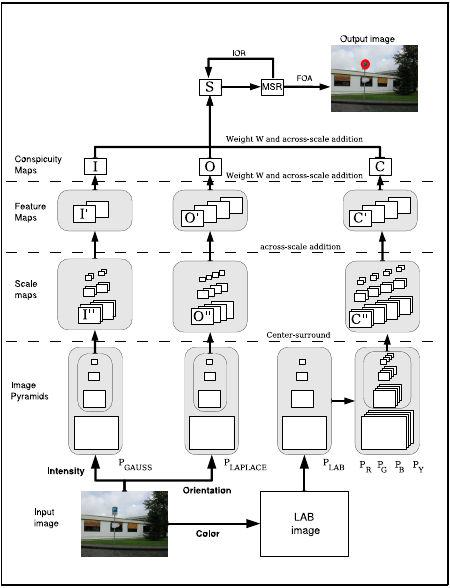
\includegraphics[width=0.6\linewidth]{img/vocus.png}
\end{center}
\caption{Componente \tit{bottom-up} do VOCUS.}
\label{fig:vocus}
\end{figure}

\subsubsection{Extração de \tit{features}}
No VOCUS, os seguintes mapas de características são extraídos de uma imagem:
luminância, luminância invertida, vermelho, verde, amarelo, azul,
orientações vertical, horizontal, 45\degree e 135\degree.
Os de luminância e cor podem ser extraídos pela conversão da imagem para o
espaço de cor LAB e as orientações são extraídas através de filtros de Gabor.

\subsubsection{Extração de saliência}

Para cada mapa extraído, a saliência é calculada usando-se o mecanismo de
\tit{center-surround}~\cite{Frintrop2006}:
uma operação que basicamente extrai contrastes fortes
do mapa, dando intensidades de pixel altas para essas regiões.
O \tit{center-surround} pode ser aplicado por meio da convolução de um
\tit{kernel} apropriado na imagem.
Tal \tit{kernel} pode ter tamanho variado, mas a soma de seus valores deve
ser zero, o centro deve ter positivo e a vizinhança deve ter valores
negativos.
\begin{figure}[H]
\begin{center}
		\begin{tabular} {ccc}
            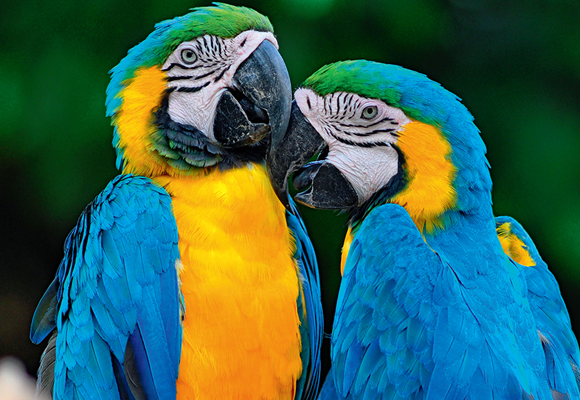
\includegraphics[width=0.3\linewidth]{img/arara.jpg}
            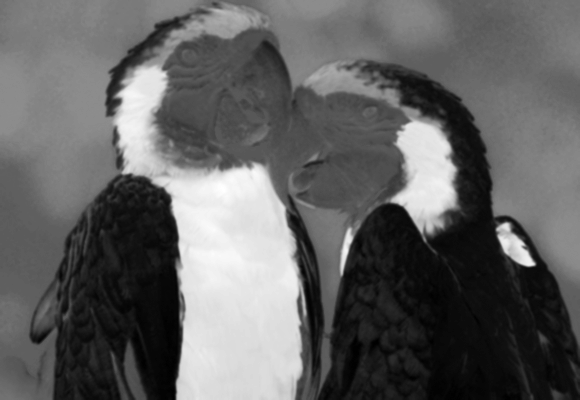
\includegraphics[width=0.3\linewidth]{img/arara_y.png}
            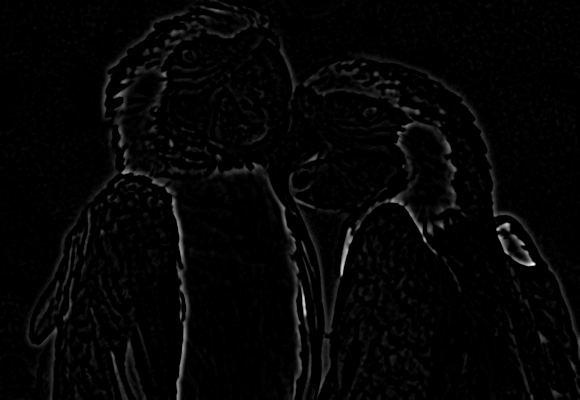
\includegraphics[width=0.3\linewidth]{img/arara_y_cs.png}
		\end{tabular}
\end{center}
\caption{À esquerda, a imagem original. No centro, seu mapa de oponência
amarelo-azul. À direita, o resultado de \tit{center-surround}
no mapa de cor.}
\label{fig:extrfeat}
\end{figure}

\subsubsection{Mapas de saliência para cada \tit{feature}}
Para cada \tit{feature} (\eg vermelho) é calculado o \tit{center-surround}.
Isso é feito na imagem original e em diversas outras dimensões dela,
calculando-se a pirâmide da imagem. Geralmente são usados quatro níveis.
Isso é importante para capturar saliências nos mais diversos níveis de detalhe
da imagem. Uma vez calculados, todos os mapas de uma certa \tit{feature}
são redimensionados para as dimensões originais e somados, formando assim
um mapa de \tit{feature}.

\subsubsection{Normalização}
Uma vez calculados os mapas para cada \tit{feature} (vermelho,
orientação horizontal, etc.), é preciso fazer uma normalização nos mesmos.
Isso se deve ao fato de que, se há grande frequência de picos de saliência
no mapa de vermelho, por exemplo, estes picos não devem ter grande importância uma vez que se
deseja identificar regiões salientes com relação à imagem como um todo (global).
Assim, para cada mapa é calculado um peso de normalização.

São diversos os critérios desenvolvidos, como: número de máximos locais,
densidade de máximos locais, espalhamento espacial dos máximos.
Uma análise das alternativas não mostrou muitas diferenças no desempenho,
então opta-se pelo método mais simples, por padrão, que é o número de máximos
locais. Isso pode ser obtido por limiar \tit{Otsu}, seguido de um algoritmo
de componentes conexos para contar os máximos locais.

\subsubsection{Mapas de saliência para cada \tit{feature}}
Uma combinação hierárquica dos mapas é feita após as normalizações.
No final dessa operação, há três mapas: cor, luminância
e orientação.
Eles são formados simplesmente somando e normalizando suas instâncias:
o de cor, por exemplo, é formado pela soma dos mapas de saliência de
vermelho, verde, amarelo e azul. A Figura \ref{fig:maps} apresenta os mapas extraídos para cada uma das dimensões descritas.
\begin{figure}[H]
\begin{center}
		\begin{tabular} {ccc}
            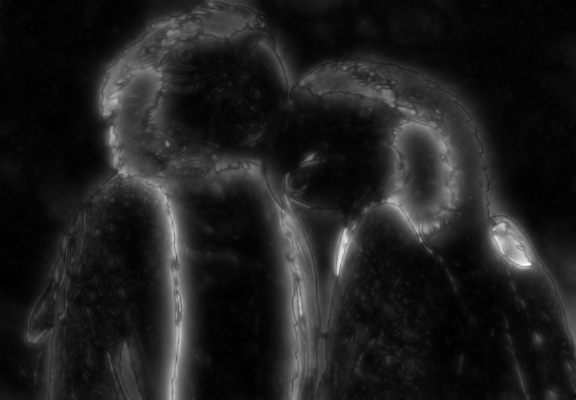
\includegraphics[width=0.3\linewidth]{img/arara_col_map.png}
            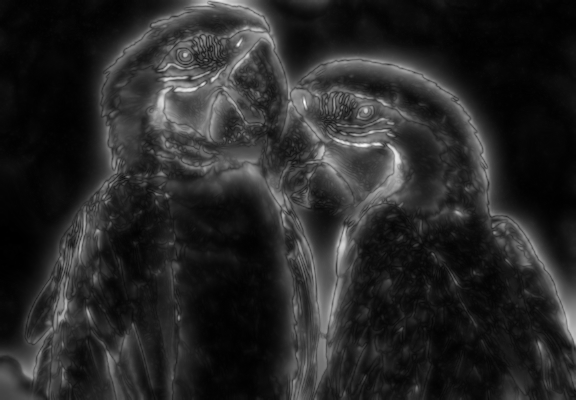
\includegraphics[width=0.3\linewidth]{img/arara_cst_map.png}
            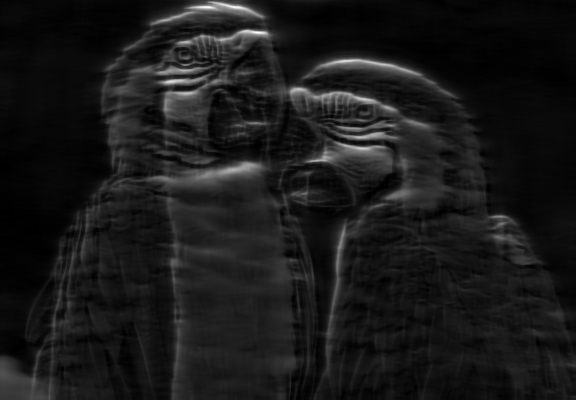
\includegraphics[width=0.3\linewidth]{img/arara_ort_map.png}
		\end{tabular}
\end{center}
\caption{Mapas de saliência da Figura original~\ref{fig:extrfeat}.
    Esquerda: mapa de cor. Centro: mapa de luminância. Direita: mapa de
orientação.}
\label{fig:maps}
\end{figure}

\subsubsection{Combinação final}
Para composição do mapa de saliência global, um peso é atribuído para cada mapa de saliência (cor, luminância, orientação) e então eles são somados e normalizados. Nos testes feitos, obteve-se
melhores resultados dando peso maior para a cor e menor para a orientação.
Nos exemplos aqui apresentados, os pesos são 2, 1, 0.1 para cor, luminância e orientação,
respectivamente.

\subsubsection{Implementação}
Todas as etapas do modelo descritas aqui foram implementadas.
A linguagem utilizada foi \tit{Python}, usando-se \tit{OpenCV} e \tit{numpy}.
O código está disponível publicamente em ~\cite{att}.

\subsection{Modelo atencional com \tit{Deep Learning}}
A tarefa de detecção de saliência visual torna-se especialmente difícil em
imagens normais não sintéticas, onde há diversos componentes potencialmente
chamativos e relações complexas de contraste e cor.
Um significativo aumento no desempenho dos modelos ocorreu quando começou-se
a usar técnicas de \tit{Deep Learning} para a tarefa.

Modelos como \emph{Salicon}~\cite{jiang_2015} demonstraram que o uso de redes
neurais convolucionais com
pesos inicializados de redes utilizadas para classificação, como a
\emph{VGG-16}~\cite{zisserman_2014},
poderiam levar à mapas de saliência visual muito similares àqueles
gerados por humanos.
A \emph{ML-Net}~\cite{cornia_2016} usa a saída de diferentes camadas da
\emph{VGG-16}, combinado-as em várias dimensões e diferentes níveis de
abstração enquanto a \emph{DeepFix}~\cite{kruthiventi_2015} estende um modelo pré-treinado com
novos layers que consideram \tit{features} globais e \tit{center bias}. Finalmente, 
a \emph{Salnet}~\cite{pan_2016} explora dois modelos bastante simples mas
com bons resultados.

O grande problema dos modelos atuais que usam \tit{Deep Learning} é que estes
são custosos, em geral porque muitos usam redes treinadas para tarefas que não
são originalmente de detecção de saliência visual, como classificação, por exemplo.
Tais redes são feitas para classificar milhares de objetos, o que requer
muitos parâmetros. Considerando o nosso objetivo de utilizar o modelo em sistemas embarcados em robôs reais, buscamos um modelo que seja eficiente, com bons resultados e computacionalmente menos custoso.
Para esta tarefa, exploramos diversos métodos de pré-processamento de dados
e uma arquitetura de rede neural totalmente convolucional que fossem ambos relevantes
no contexto de saliência visual. O modelo final proposto foi nomeado \tit{DeepPeek}.

\subsubsection{Arquitetura proposta}
A Figura~\ref{fig:model} mostra a arquitetura da rede neural totalmente
convolucional proposta no trabalho.
A rede extrai \tit{features} de dimensões cada vez menores da imagem de
entrada, sendo composta de quatro blocos principais:

\begin{figure}[H]
    \centering
    \def\svgwidth{0.9\columnwidth}
    \input{./img/model.pdf_tex}
    \label{fig:model}
    \caption{Visão geral da arquitetura proposta.
        Tamanhos de filtros estão em formato
        largura$\times$altura\_passo.}
\end{figure}

\begin{enumerate}
    \item O primeiro nível extrai \tit{features} de baixo nível de abstração
        da imagem de entrada, de dimensões
        $W\times H \times 3$ (largura, altura, canais), usando uma única
        camada com 48 filtros de convolução com ativação ReLU seguida por
        \tit{max-pooling} que reduz a imagem por um fator de dois.
        Reduzir o número de filtros nesta camada mostrou-se prejudicial para
        o desempenho da rede, pois é importante captar informação de
        alta frequência no contexto de saliência visual.
    \item O segundo nível extrai \tit{features} de baixo/médio nível de
        abstração da entrada de dimensões $W/2 \times H/2 \times 48$
        usando duas camadas com 64 e 96 filtros de convolução, respectivamente,
        seguidos por ativação ReLU e \tit{max-pooling}.
    \item O terceiro nível extrai \tit{features} de médio/alto nível de
        abstração da entrada de dimensões $W/4 \times H/4 \times 96$ usando
        quatro filtros de convolução.
        As primeiras duas camadas têm 128 filtros cada e as duas últimas
        têm 144 filtros cada. Toda camada de convulução é seguida de ReLU.
        \tit{Max-pooling} acontece no final.
        Um grande número de filtros neste nível mostrou-se importante para
        o desempenho da rede.
    \item O quarto e último nível é composto de oito blocos \tit{inception}
        que extraem \tit{features} de alto nível de abstração da entrada
        com dimensões $W/8 \times H/8 \times 144$.
        Um número elevado de blocos mostrou-se importante.
        Uma convolução de $1 \times 1$ no final faz uma combinação linear
        dos mapas de saída dos blocos \tit{inception}, seguida por ReLU,
        produzindo o mapa final de saliência de dimensões
        $W/8 \times H/8 \times 1$.
        O mapa é redimensionado para as dimensões originais da imagem
        com interpolação bicúbica.
\end{enumerate}

A Figura \ref{fig:newinception} ilustra a arquitetura
\tit{inception}~\cite{szegedy_2014}
usada em cada bloco onde são aplicados
filtros de dimensões $5 \times 5$, $3 \times 3$
(ambos precedidos por convoluções $1\times 1$ para redução de dimensionalidade)
, $1 \times 1$, e \tit{max-pooling} de tamanho $3 \times 3$.
Cada um desses filtros é aplicado em paralelo da mesma entrada e as saídas
são concatenadas no final.
\tit{Inception} permite que a rede use informação de diferentes resoluções
espaciais assim como de camadas anteriores (mais baixo nível),
aspectos importantes no contexto de saliência visual.

\begin{figure}[H]
    \centering
    \def\svgwidth{0.57\linewidth}
    \input{./img/inception.pdf_tex}
    \caption{Bloco \tit{inception}}.
   \label{fig:newinception}
\end{figure}

A rede tem um total de $3717841$ parâmetros, um número muito baixo comparado
a outros modelos.
A tabela \ref{table:inception} detalha os números de filtros para cada
bloco \tit{inception} utilizado.

\begin{table}[H]
\centering
	\small
\label{table:inception}
\caption{Número de filtros usado em cada bloco \tit{inception}.}
\begin{tabular}{|c|c|c|c|c|c|c|}
	\hline
    Bloco & pool & conv 1$\times$1 & 3$\times$3 reduce &
    conv 3$\times$3 & 5$\times$5 reduce & conv 5$\times$5\\
    \hline
    1 & 96 & 128 & 96 & 192 & 58 & 96\\
    \hline
    2 & 64 & 128 & 80 & 160 & 24 & 48\\
    \hline
    3 & 64 & 128 & 80 & 160 & 24 & 48\\
    \hline
    4 & 64 & 128 & 96 & 192 & 28 & 56\\
    \hline
    5 & 64 & 128 & 96 & 192 & 28 & 56\\
    \hline
    6 & 64 & 128 & 112 & 224 & 32 & 64\\
    \hline
    7 & 64 & 128 & 112 & 224 & 32 & 64\\
    \hline
    8 & 112 & 160 & 128 & 256 & 40 & 80\\
    \hline
\end{tabular}
\end{table}

\subsubsection{Implementação}
A rede proposta foi implementada usando-se \emph{Theano} \texttt{0.9.0.dev}
com \emph{Lasagne} \texttt{0.2.dev1}
em uma máquina com \emph{Ubuntu 16.04 LTS} e
kernel \emph{Linux} \texttt{4.8.0-54-generic}.
O treinamento foi feito em uma GPU \emph{NVIDIA GTX 1080} e o código está
disponível em \texttt{https://goo.gl/WzpyYJ}.

\subsubsection{Treinamento}
Durante o treinamento, as imagens foram redimensionadas para
$320\times240\times3$.
Cada imagem é normalizada por canal pela subtração da média e
divisão pelo desvio padrão.
Além disso, dois aspectos são importantes nesta etapa:
1) o uso de normalização por imagem, ao invés de pelo \tit{dataset}, e 2) a
conversão do espaço de cor das imagens para LAB (ao invés do comum RGB).
Esses procedimentos não foram encontrados na literatura, mas são consideradas
importantes no contexto de saliência visual.
A normalização por imagem usa mais informação do contexto global da imagem, e
\emph{VOCUS} cita que o espaço de cor LAB é mais fiel ao sistema visual humano
uma vez que ele contém mapas vermelho-verde, amarelo-azul e mapas de
luminância.
Conjectura-se que tais mapas facilitam a extração de \tit{features}
importantes.
Experimentos preliminares mostraram que as duas técnicas resultam em melhor
desempenho da rede.

A função objetivo a se minimizar foi
o coeficiente de correlação entre o mapa de saliência \tit{ground-truth} $G$
e o mapa previsto $P$:
$$CC(P, G) = \frac{cov(P, G)}{(\sigma(P)\sigma(G))}$$
Tal função de custo é considerada apropriada pois ela penaliza simetricamente
falsos positivos e negativos.

Dois \tit{datasets foram utilizados}:
\emph{SALICON} e \emph{Judd}.
A rede foi treinada usando-se \tit{Stochastic Gradient Descent}
com Momento de \tit{Nesterov} de $0.9$.
Salicon foi primeiramente usado com \tit{data augmentation} espelhando-se
imagens horizontalmente e verticalmente.
O treinamento ocorreu por 5 épocas com \tit{learning rate} de $0.009$
e então por 3 épocas com \tit{learning rate} de $0.001$.
Mudou-se então para o \tit{dataset} Judd.
O treinamento ocorreu por mais uma época, com \tit{learning rate} de
$3\times10^{-5}$ e regularização L2 de $10^{-4}$.
Os tamanhos de batch foram 10 para SALICON e 2 para Judd.
O processo de treinamento todo levou cerca de duas horas e meia.

\section{Resultados}
As Figuras~\ref{fig:att} e ~\ref{fig:preds} ilustram, respectivamente,
mapas gerados pelos modelos \tit{att} (tradicional) e \tit{DeepPeek}
(com \tit{Deep Learning}).
A tabela ~\ref{table:results} mostra os resultados obtidos pela submissão
dos modelos ao \tit{MIT300 benchmark} em comparação com alguns dos melhores
modelos do ranking.

\begin{figure}[H]
\begin{center}
        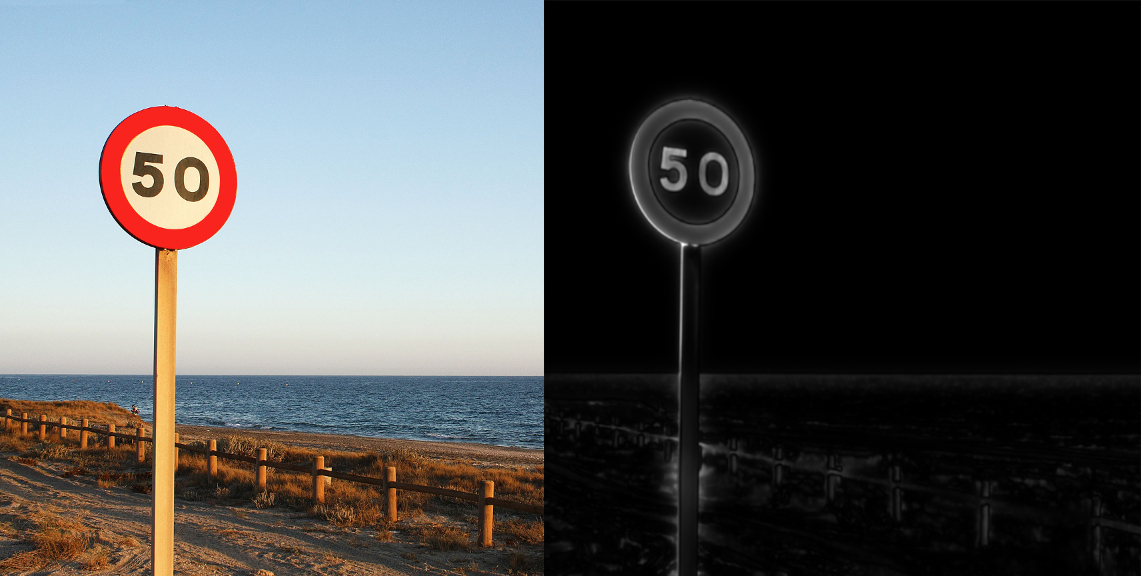
\includegraphics[width=0.6\linewidth]{img/att.png}
\end{center}
\caption{Mapa de saliência final para uma figura gerado pelo modelo \tit{att}.
    À esquerda, a imagem original. À direita, o mapa de saliência final.}
\label{fig:att}
\end{figure}

\begin{figure}[H]
\begin{center}
		\begin{tabular} {ccc}
        Imagem & Ground-truth & DeepPeek\\
		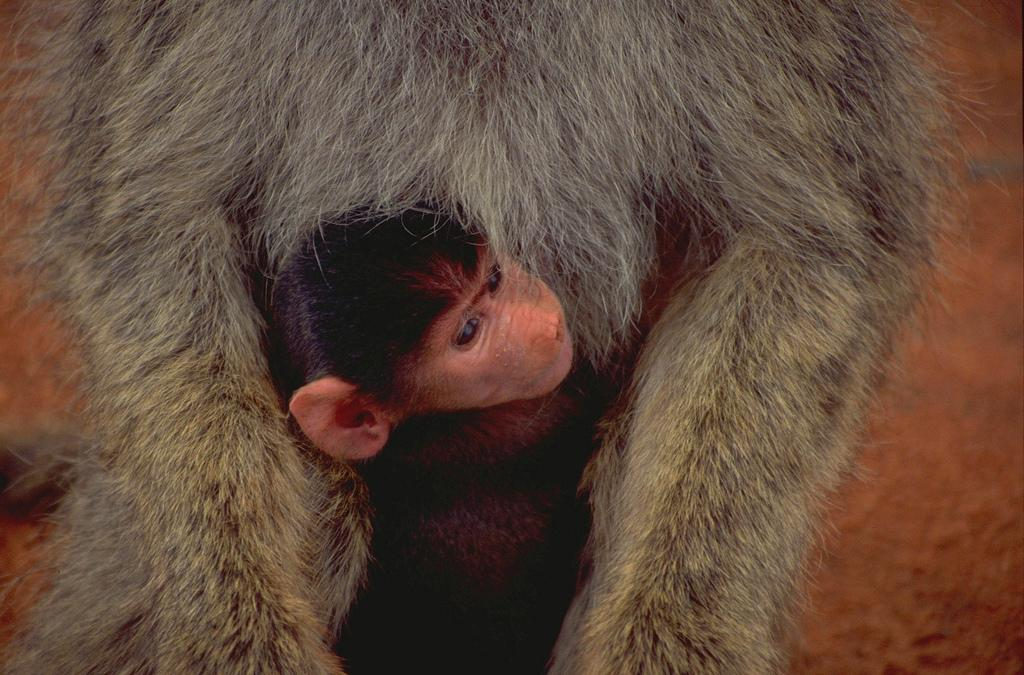
\includegraphics[width=0.19\textwidth]{./img/monkey_s.jpg} &
        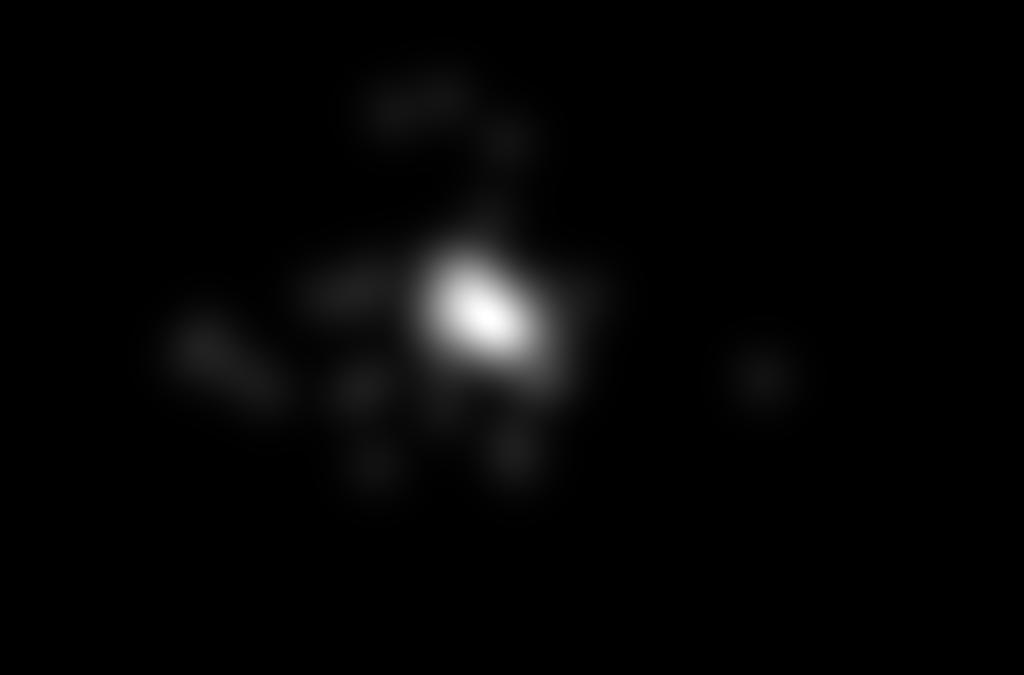
\includegraphics[width=0.19\textwidth]{./img/monkey_gt.jpg} &
		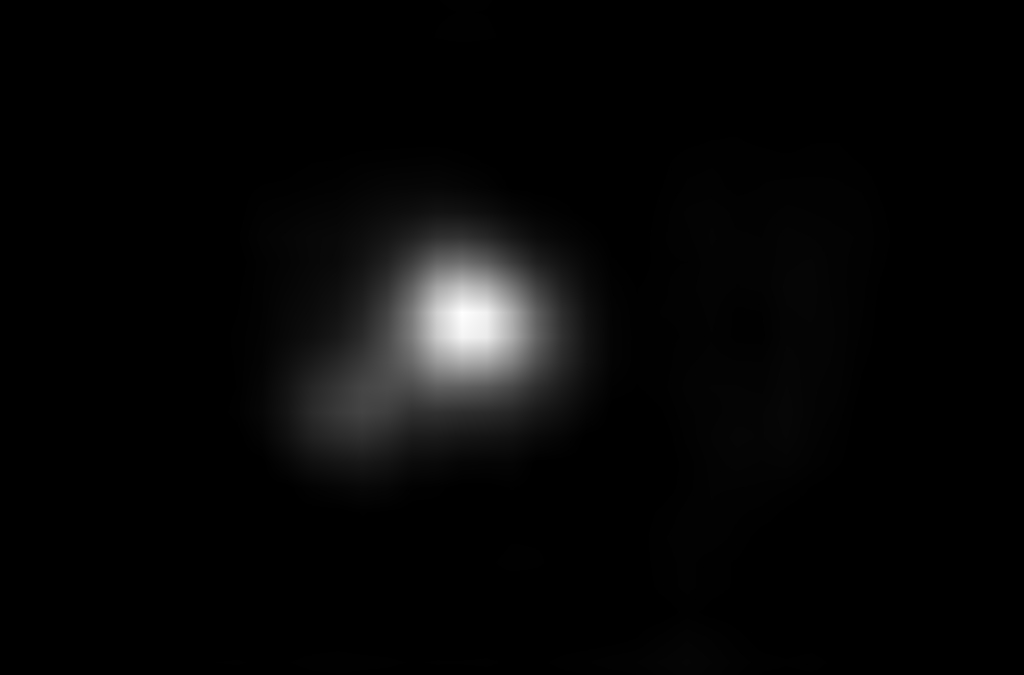
\includegraphics[width=0.19\textwidth]{./img/monkey_m.jpg}\\
		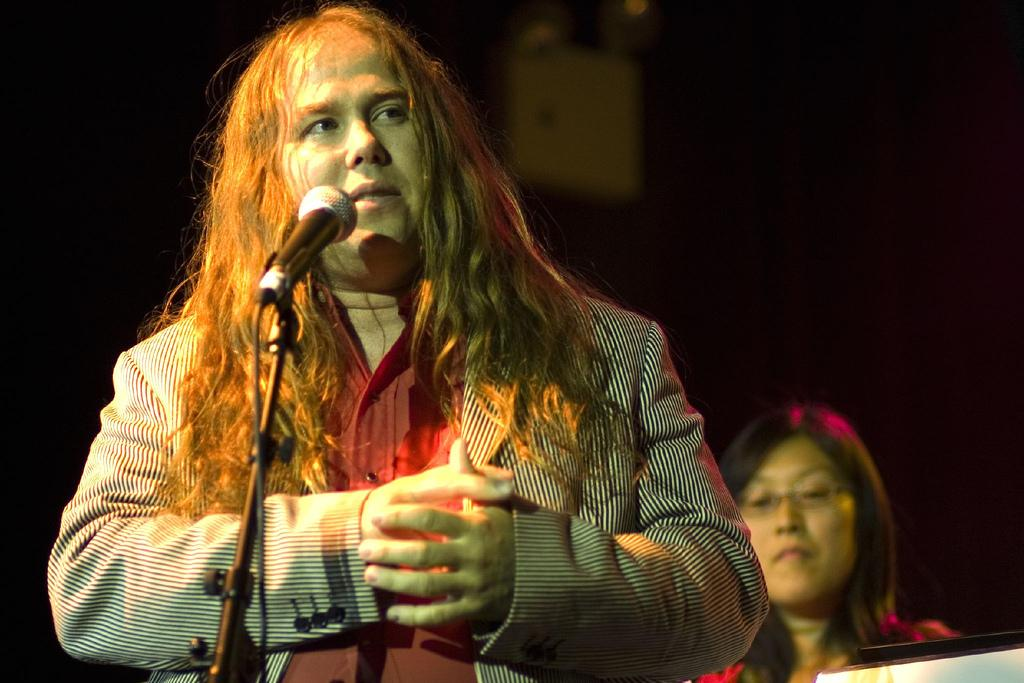
\includegraphics[width=0.19\textwidth]{./img/person_s.jpg} &
        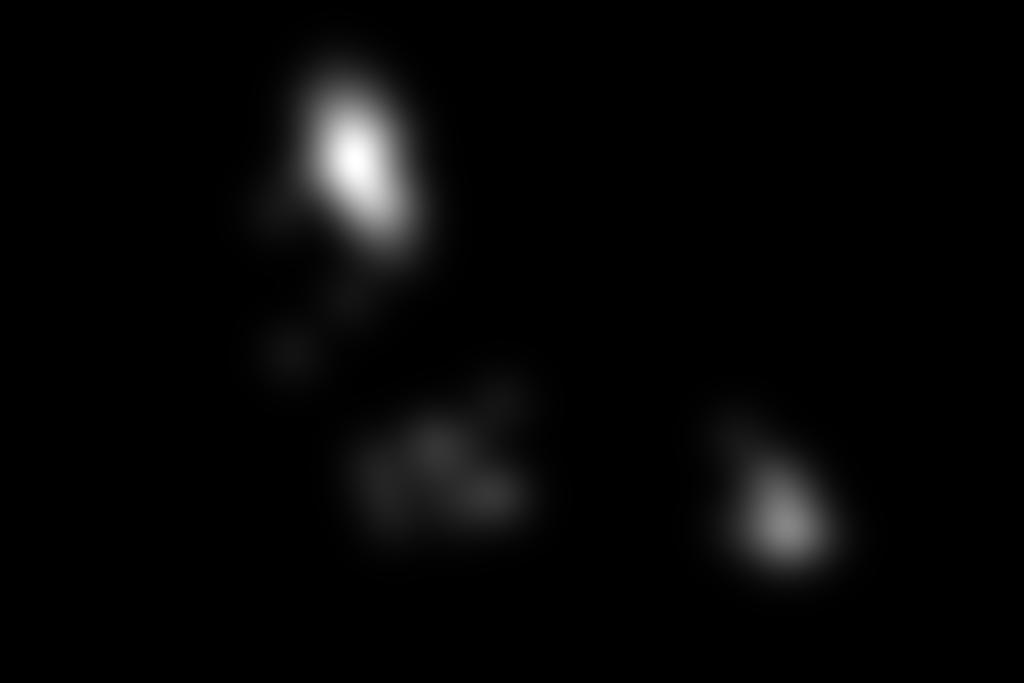
\includegraphics[width=0.19\textwidth]{./img/person_gt.jpg} &
		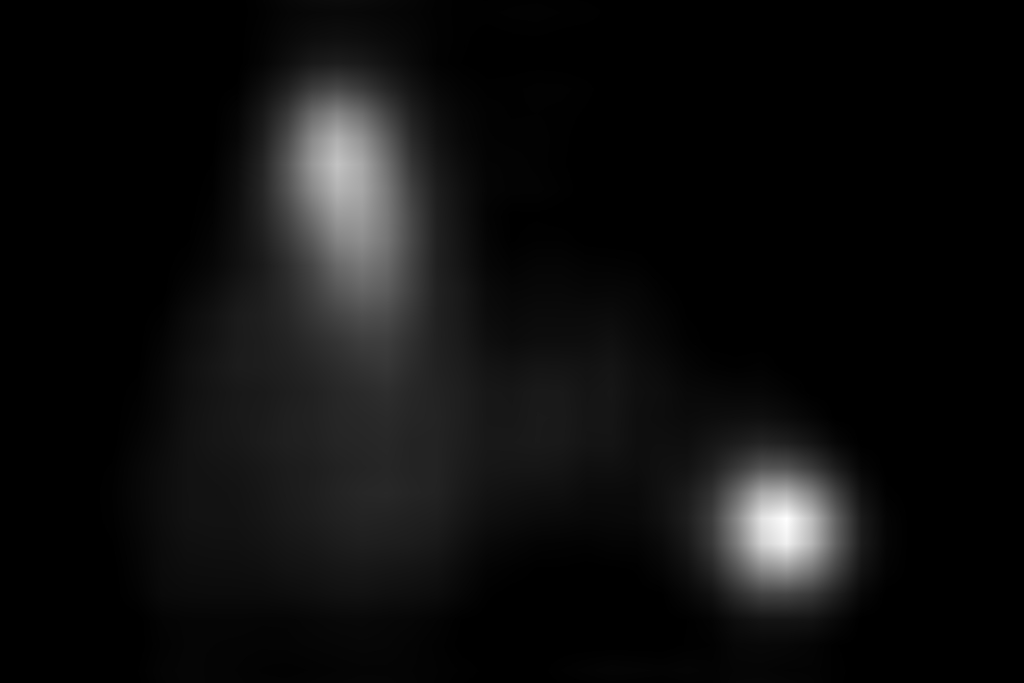
\includegraphics[width=0.19\textwidth]{./img/person_m.jpg}\\
		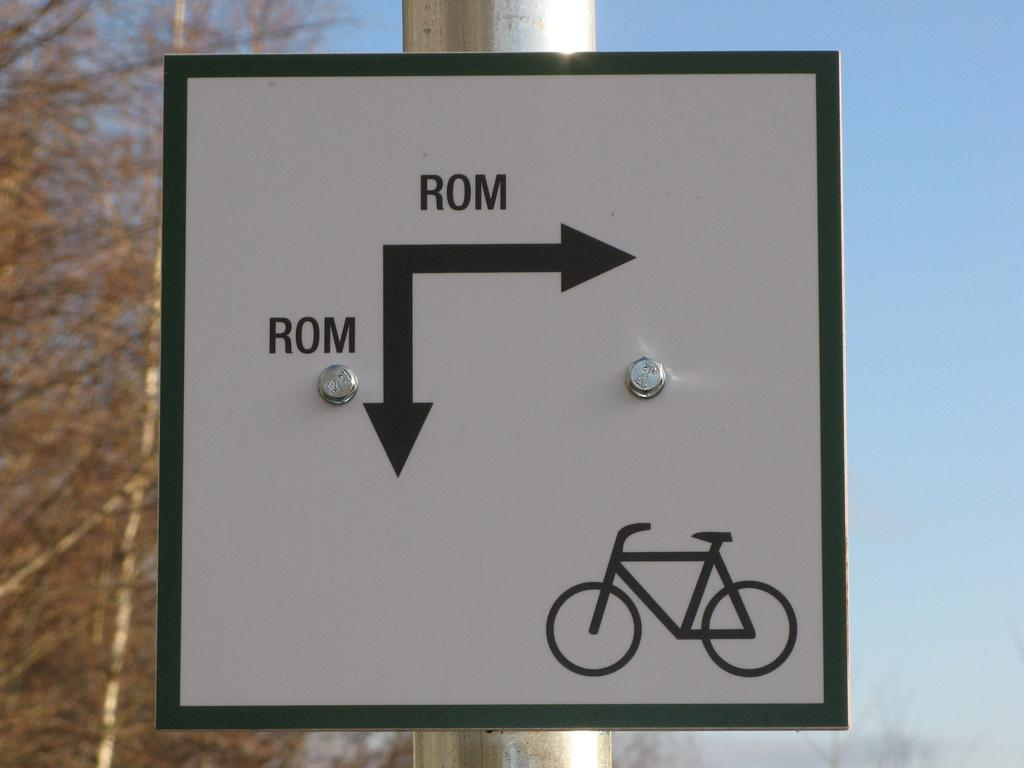
\includegraphics[width=0.19\textwidth]{./img/sign_s.jpg} &
        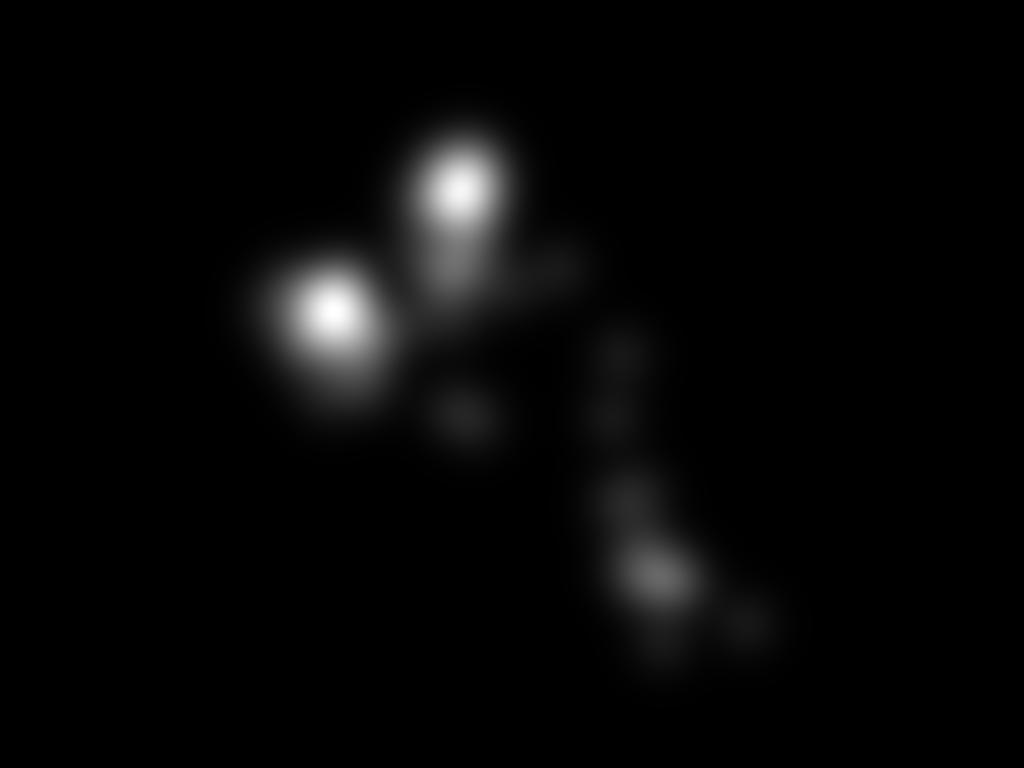
\includegraphics[width=0.19\textwidth]{./img/sign_gt.jpg} &
		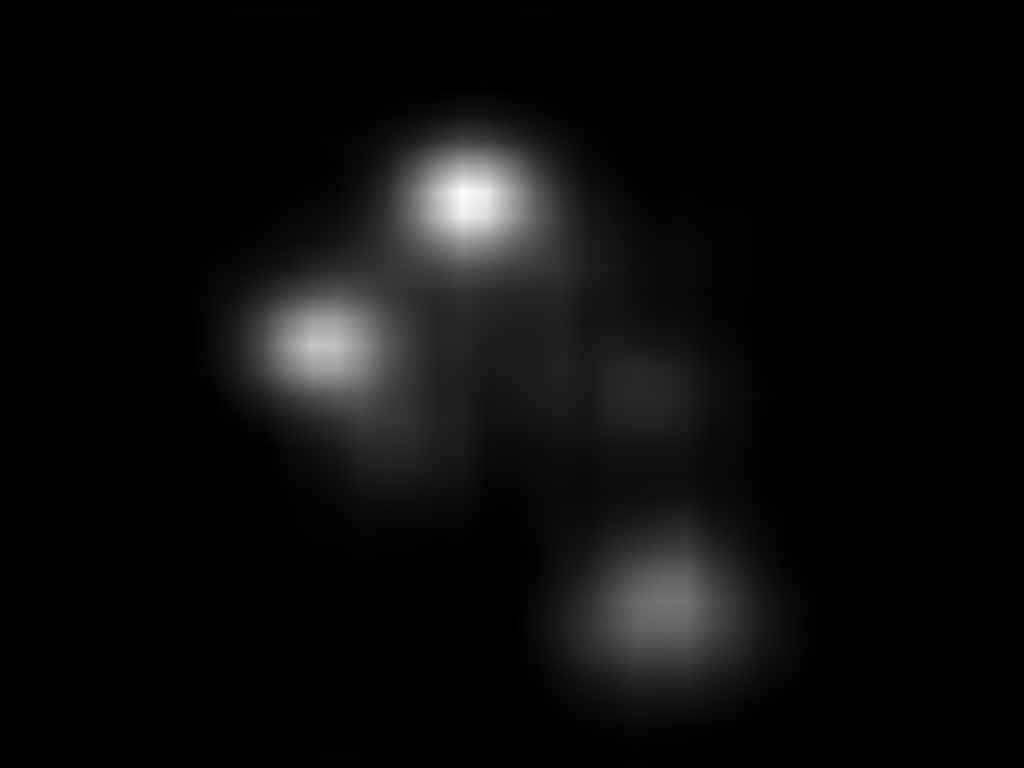
\includegraphics[width=0.19\textwidth]{./img/sign_m.jpg}\\
		\end{tabular}
\end{center}
\caption{Exemplos de mapas de saliência gerados pelo modelo \tit{DeepPeek}.}
\label{fig:preds}
\end{figure}

\begin{table}[!htb]
	\small
    \centering
    \label{table:results}
    \caption{Comparação de resultados com modelos propostos e melhores
        modelos no \emph{MIT300 benchmark}.}
    \begin{tabular}{|c|c|c|c|c|c|c|}
        \hline
        Modelo & Num. parâmetros & AUC-Judd $\uparrow$ & CC $\uparrow$
            & NSS $\uparrow$ & Sim $\uparrow$ & EMD $\downarrow$\\
        \hline
        \emph{DeepFix} & $\approx$16.7 milhões & 0.87 & 0.78
            & 2.26 & 0.67 & 2.04\\
        \hline
        \emph{Salicon} & $\approx$14.7 milhões & 0.87 & 0.74 & 2.12
            & 0.60 & 2.62\\
        \hline
        \textbf{DeepPeek} & \textbf{3.72 milhões} & \textbf{0.85} &
        \textbf{0.71} & \textbf{1.98} & \textbf{0.62} & \textbf{2.37}\\
        \hline
        \emph{ML-Net} & $\approx$15.4 milhões & 0.85 & 0.69 & 2.07 & 0.60
            & 2.53\\
        \hline
        \emph{SalNet} & 25.8 milhões & 0.83 & 0.57 & 1.51 & 0.52 & 3.31\\
        \hline
        \textbf{att} & - & \textbf{0.62} &
        \textbf{0.12} & \textbf{0.34} & \textbf{0.33} & \textbf{5.28}\\
        \hline
    \end{tabular}
\end{table}

Nota-se que o \tit{DeepPeek} obteve resultados muito similares aos dos
melhores modelos atuais, com cerca de um quarto do número de parâmetros dos
outros modelos.

\section{Conclusões}
Neste trabalho, foram explorados dois modelos de saliência visual:
\tit{att}, um modelo baseado no modelo VOCUS,
que usa técnicas de extração de um conjunto pré-selecionado de \tit{features};
e \tit{DeepPeek}, uma rede neural totalmente convolucional com foco em
eficiência.

A tabela ~\ref{table:results} mostra que o modelo \tit{att} tem desempenho
muito abaixo dos melhores modelos atuais.
Os resultados indicam que as técnicas atuais de aprendizado
de filtros de extração de \tit{features} são de fato necessárias para
um bom desempenho na tarefa de detecção de saliência visual.

O modelo \tit{DeepPeek} mostra um bom desempenho, sendo comparável
ao dos melhores modelos atualmente, tendo apenas cerca de $1/4$ do número
de parâmetros dos outros modelos.
Assim, conclui-se que um modelo eficiente foi obtido com sucesso.
O desenvolvimento de uma arquitetura completamente dedicada à saliência visual,
juntamente com técnicas de pré-processamento de dados especialmente para
o contexto de saliência, mostraram-se importantes para o resultado obtido.

\subsection{Próximos passos}
Planeja-se, em futuros trabalhos, estender o modelo \tit{DeepPeek} para
que o mesmo seja usado para a detecção de saliência visual em vídeos.
Tal domínio ainda é pouco explorado por modelos atuais e requer a consideração
de aspectos novos.
Saliência em vídeo é importante para o uso do sistema por robôs móveis.

\section{Publicações derivadas do trabalho}
O trabalho desenvolvido na obtenção do modelo \tit{DeepPeek} resultou em um
artigo, \tit{Efficient Visual Attention with Deep Learning}~\cite{myarticle},
publicado no WTD2017~\cite{wtd2017} do Instituto de Computação da Unicamp.
O artigo e a apresentação do mesmo resultaram na premiação de
\tbf{melhor trabalho de Iniciação Científica} do Instituto de Computação. Os resultados finais serão submetidos a uma publicação de referência na área.

\printbibliography

%\end{multicols}
\end{document}
